\documentclass[notes,11pt, aspectratio=169]{beamer}

\usepackage{pgfpages}
% These slides also contain speaker notes. You can print just the slides,
% just the notes, or both, depending on the setting below. Comment out the want
% you want.
\setbeameroption{hide notes} % Only slide
%\setbeameroption{show only notes} % Only notes
%\setbeameroption{show notes on second screen=right} % Both

\usepackage{helvet}
\usepackage[default]{lato}
\usepackage{array}


\usepackage{tikz}
\usepackage{verbatim}
\setbeamertemplate{note page}{\pagecolor{yellow!5}\insertnote}
\usetikzlibrary{positioning}
\usetikzlibrary{snakes}
\usetikzlibrary{calc}
\usetikzlibrary{arrows}
\usetikzlibrary{decorations.markings}
\usetikzlibrary{shapes.misc}
\usetikzlibrary{matrix,shapes,arrows,fit,tikzmark}
\usepackage{amsmath}
\usepackage{mathpazo}
\usepackage{hyperref}
\usepackage{lipsum}
\usepackage{multimedia}
\usepackage{graphicx}
\usepackage{multirow}
\usepackage{graphicx}
\usepackage{dcolumn}
\usepackage{booktabs,tabularx}
\usepackage{bbm}
\usepackage{hyperref}
\newcolumntype{d}[0]{D{.}{.}{5}}

\usepackage{changepage}
\usepackage{appendixnumberbeamer}
\newcommand{\beginbackup}{
   \newcounter{framenumbervorappendix}
   \setcounter{framenumbervorappendix}{\value{framenumber}}
   \setbeamertemplate{footline}
   {
     \leavevmode%
     \hline
     box{%
       \begin{beamercolorbox}[wd=\paperwidth,ht=2.25ex,dp=1ex,right]{footlinecolor}%
%         \insertframenumber  \hspace*{2ex} 
       \end{beamercolorbox}}%
     \vskip0pt%
   }
 }
\newcommand{\backupend}{
   \addtocounter{framenumbervorappendix}{-\value{framenumber}}
   \addtocounter{framenumber}{\value{framenumbervorappendix}} 
}


\usepackage{graphicx}
\usepackage[space]{grffile}
\usepackage{booktabs, fontawesome}

% These are my colors -- there are many like them, but these ones are mine.
\definecolor{blue}{RGB}{0,114,178}
\definecolor{red}{RGB}{213,94,0}
\definecolor{yellow}{RGB}{240,228,66}
\definecolor{green}{RGB}{0,158,115}

\hypersetup{
  colorlinks=false,
  linkbordercolor = {white},
  linkcolor = {blue}
}


%% I use a beige off white for my background
\definecolor{MyBackground}{RGB}{255,253,218}

%% Uncomment this if you want to change the background color to something else
%\setbeamercolor{background canvas}{bg=MyBackground}

%% Change the bg color to adjust your transition slide background color!
\newenvironment{transitionframe}{
  \setbeamercolor{background canvas}{bg=MyBackground}
  \begin{frame}}{
    \end{frame}
}

\setbeamercolor{frametitle}{fg=blue}
\setbeamercolor{title}{fg=black}
\setbeamertemplate{footline}[frame number]
\setbeamertemplate{navigation symbols}{} 
\setbeamertemplate{itemize items}{-}
\setbeamercolor{itemize item}{fg=blue}
\setbeamercolor{itemize subitem}{fg=blue}
\setbeamercolor{enumerate item}{fg=blue}
\setbeamercolor{enumerate subitem}{fg=blue}
\setbeamercolor{button}{bg=MyBackground,fg=blue,}

% If you like road maps, rather than having clutter at the top, have a roadmap show up at the end of each section 
% (and after your introduction)
% Uncomment this is if you want the roadmap!
% \AtBeginSection[]
% {
%    \begin{frame}
%        \frametitle{Roadmap of Talk}
%        \tableofcontents[currentsection]
%    \end{frame}
% }
\setbeamercolor{section in toc}{fg=blue}
\setbeamercolor{subsection in toc}{fg=red}
\setbeamersize{text margin left=1em,text margin right=1em} 

\newenvironment{wideitemize}{\itemize\addtolength{\itemsep}{10pt}  \setlength\itemsep{.5em}}{\enditemize}

\title[]{How do borrowers find their banks? \\ \vspace{.2cm} The value of individuals in bank relationship formation}
\author[PGP]{Marco Ceccarelli \inst{1}, Christoph Herpfer \inst{2}, Steven Ongena \inst{1}}
\institute[FRBNY]{\small{\begin{tabular}{c c c}
 \inst{1} Swiss Finance Institute and UZH & \hspace*{0.01cm}  & \inst{2} Emory University, Goizueta Business School  \\ \\
        \vspace*{0.5cm}
\includegraphics[scale=0.1]{./figures/sfi_logo}   & \hspace*{0.1cm}  &  
\includegraphics[scale=0.20]{./figures/GBS_hz_280} \vspace{.2cm} \\ 
\multicolumn{3}{c}{SFI Research Days} 
\end{tabular}}}

\date{June 9, 2020}


\begin{document}

%%% TIKZ STUFF
\tikzset{   
        every picture/.style={remember picture,baseline},
        every node/.style={anchor=base,align=center,outer sep=1.5pt},
        every path/.style={thick},
        }
\newcommand\marktopleft[1]{%
    \tikz[overlay,remember picture] 
        \node (marker-#1-a) at (-.3em,.3em) {};%
}
\newcommand\markbottomright[2]{%
    \tikz[overlay,remember picture] 
        \node (marker-#1-b) at (0em,0em) {};%
}
\tikzstyle{every picture}+=[remember picture] 
\tikzstyle{mybox} =[draw=black, very thick, rectangle, inner sep=10pt, inner ysep=20pt]
\tikzstyle{fancytitle} =[draw=black,fill=red, text=white]
%%%% END TIKZ STUFF

% Title Slide
\begin{frame}
  \maketitle
\end{frame}
\note[itemize]{
\item INTRO SLIDE
\item Thanks for being here + coauthors 
\item In this paper we attempt to fill an important hole in the relationship lending literature: how banks and borrowers match. We will argue that the individual bankers play a crucial role in this matching, and then we will ask how do frictions in the labor market of these bankers spill over in the capital markets and show that these frictions affect firms' financing.
\item Practitioners always stress how important personal relationships are in lending, and there is ample anecdotal evidence. Consider this newspaper article that makes exactly our point:
%Let me start by providing some anecdotal evidence that bankers do indeed matter and that when they jump ship to a competing bank they take their client portfolio with them. 
}

%%%%%%%%%%%%%%%%%%%%%%%%%%%%%%%%%%%%%%%
% BIG PICTURE QUESTION AND MOTIVATION
%%%%%%%%%%%%%%%%%%%%%%%%%%%%%%%%%%%%%%%
\section{Big picture}
\begin{frame}{Anecdotal evidence}
\centering
  \faQuoteLeft~ [CEO Dan Ariens] approached his lender, LaSalle Bank, to see if it would ramp up his credit line. But LaSalle [\ldots] would never get the additional business. \\ \vspace{.5cm} 
 \onslide<2->{  Ariens, in fact, ended up \textcolor{red}{moving nearly all of his banking relationships to PrivateBancorp.} The Chicago-based bank \textcolor{red}{hired 56 managing directors} in the fourth quarter, \textcolor{red}{most of them from LaSalle}, and posted a 12\% increase in loans compared with the year-ago quarter. \\ \vspace{.5cm} }
 \onslide<3->{  \textbf{\textcolor{red}{ ``It felt natural to stay with the people we knew,'' }} [the CEO] said.~\faQuoteRight \\ \vspace{.5cm} } \hfill  (Chicago Tribune, February 18, 2008) 

 \end{frame}


%%%%%%%%%%%%%%%%%%%%%%%%%%%%%%%%%%%%%%%
% MOTIVATION AND PREVIEW
%%%%%%%%%%%%%%%%%%%%%%%%%%%%%%%%%%%%%%%
\begin{frame}{Motivation}
\textcolor{red}{Lending relationships:} 
\begin{wideitemize}
  \item have a large impact on borrowers, e.g., impacting both the availability (Ioannidou, Ongena (JF, 2010)) and pricing of credit (Khwaja,  Mian (AER, 2008))
  \item are a channel through which shocks to the banking system are transmitted to the real sector (e.g. Chodorow-Reich (QJE, 2014), Chodorow-Reich, Falato (2019))
\end{wideitemize} \vspace{.3cm}

\onslide<2->{ 
\begin{center}
How are these relationships formed? \textcolor{red}{How do banks and borrowers actually match?} \\ \vspace{.3cm}
\end{center}
}

\onslide<3->{ 
\textcolor{red}{The role of bankers:} 
}
\begin{wideitemize}
\onslide<3->{ 
  \item bankers are the source of soft information about borrower (Berger, Udell (EJ, 2002))
} \onslide<4->{ 
  \item hence, they ought to play a \textcolor{red}{key role in matching borrowers to banks}
} \onslide<5->{ 
 \item and frictions in the labor market for bankers have \textcolor{red}{consequences in capital markets}
} \end{wideitemize} \vspace{.2cm}
\end{frame}
\note[itemize]{
\item MOTIVATION
\item Let me try to convince you that the question we are asking is indeed an important one. 
\item We know banking relationships are very important bc they change loan terms and loan availability and because they are a channel through which shocks in the financial sector are transmitted to the real economy
\item However, there is little evidence on how these relationships are formed - and more specifically - on how banks and borrowers actually match
\item We start with the observation that bankers are (1) the source of soft information about the borrower. Hence (2) it seems reasonable to assume that they ought to play a key role in the matching of borrowers and banks. 
\item (3) Finally, we will argue that frictions in the labor market for bankers have real consequences in capital market decisions of firms. 
}


%%%%%%%%%%%%%%%%%%%%%%%%%%%%%%%%%%%%%%%
\begin{frame}{Preview of findings}
\begin{enumerate} 

\item Banks recognize the ability of bankers to bring clients and poach them strategically:
\begin{wideitemize}
\onslide<2->{ 
      \item Bankers are more likely to get poached by competitors if 
      \begin{itemize}
      			\item they have \textcolor{red}{more clients} 
      			\item they have \textcolor{red}{more valuable} clients
      			\item they are the \textcolor{red}{only relationship banker} for clients
		\end{itemize}  
    }
\end{wideitemize} \vspace{.2cm}

\onslide<3->{ 
\item Bankers succeed in bringing their clients with them 
\begin{wideitemize}
  \item After a banker switches to another bank, the \textcolor{red}{likelihood of borrowers following the banker increases by 14\%} (ca. 3$\times$  uncond. average)
  \item These clients have \textcolor{red}{significant value}: Deal volume with these clients increases by 35\%
	\item New relationships are \textcolor{red}{long lasting} and extend to \textcolor{red}{other financial products}
\end{wideitemize} \vspace{.2cm}
}

\onslide<4->{ 
\item Frictions in the labor market have spillover effects into capital markets 
\begin{wideitemize}
  \item Use gender discrimination lawsuits and absence of female directors as a proxies for less female friendly cultures
  \item Banks with such culture \textcolor{red}{lose female bankers and their clients}
\end{wideitemize}
}
\end{enumerate}
\end{frame}

\note[itemize]{
\item PREVIEW OF FINDINGS
\item Our first main finding shows that banks recognize the ability of the individual bankers to bring in additional business and poach them strategically, in particular: 
\item Our second finding stresses the importance of the bankers for the new bank: Not only do they succeed in bringing their clients from the old bank with them to the new bank, but these relationships that the bank acquires have significant financial value and are long lasting
\item Finally we show that frictions from the labor market - in particular instances of bank culture that is unfriendly towards women - spill over in the capital markets. Such women-unfriendly banks are significantly more likely to lose female bankers and their clients. 
}


%%%%%%%%%%%%%%%%%%%%%%%%%%%%%%%%%%%%%%%
% LITERATURE OVERVIEW
%%%%%%%%%%%%%%%%%%%%%%%%%%%%%%%%%%%%%%%

\begin{frame}{Literature review - Relationship lending}
Relationship lending plays a key role for both banks and firms:
\begin{wideitemize}
    \onslide<1->{ 
     \item The ability of banks to create information about their borrowers is at the core of banking {\tiny\textcolor{blue}{ (e.g. Berger and Udell, JofB 1995;  Diamond, REStud 1984; Petersen and Rajan, JF 1994)}}
     \item The \textcolor{red}{soft information} of lending relationships is concentrated in individual bankers \\ {\textcolor{blue}{\tiny(e.g. Berger and Udell, EJ 2002; Liberti and Petersen, RCFS 2019; Herpfer, 2020)}} }
  \onslide<2->{ 
     \item Banking relationships influence loan conditions and availability  \\ {\tiny \textcolor{blue}{(e.g. Bharat, Dahiya, Saunders, Srinivasan, RFS 2011; Ongena and Smith, JFE 2001)}}
     \item Banking relationships transmit shocks from the financial to the real sector \\ {\tiny \textcolor{blue}{(e.g. Chava, Purnanandam, JFE 2011, Chodorow-Reich, QJE 2014, Chodorow-Reich, Falato, 2019)}}
     } 
\end{wideitemize} 

\onslide<3->{
\textcolor{red}{Therefore crucial to understand how these relationships form - we know surprisingly little !}
 \vspace{.2cm}
      \textcolor{red}{What drives the formation of relationships between firms and banks?} \\ 
      \begin{wideitemize} 
      	\item Endogenous matching between banks and borrowers {\tiny \textcolor{blue}{(Schwert, JF 2018; Petersen and Rahan, QJE 1995)}}
      	\item ``Life cycle'' of banking relationships { \textcolor{blue}{\tiny (Ioannidou and Ongena, JF 2010)}}
  \end{wideitemize} }

\end{frame}
\note[itemize]{
  \item LITERATURE REVIEW
  \item Ability of banks to create information, in particular soft information, is one of the factors that makes banks special. 
  \item Importantly, this soft information is concentrated in individual bankers. While this has been established in the theoretical literature for some time, only recently the role of the individual bankers has been shown empirically.
  \item The banking relationships are important since they influence the availability and conditions of credit and because they link the financial and the real economy 
  \item Hence, it is crucial to understand how these relationships are formed. But, we know surprisingly little!
}

\begin{frame}{Contribution - Role of bankers}

Nascent literature on commercial bankers for large U.S.\ borrowers:

\begin{wideitemize}
	\item Bankers play an important role in the lending process and form personal relationships with borrowers {\tiny \textcolor{blue}{(Bushman, Gao, Martin, Pacelli (2019), Herpfer (2020))}}
	\item Spillover from lending to bankers' labor markets	{\tiny \textcolor{blue}{(Gao, Kleiner, Pacelli (RFS, 2020))}}
	\item  Bankers curate their portfolio of clients	{\tiny \textcolor{blue}{(Frattaroli, Herpfer (2020))}}
\end{wideitemize}

\onslide<2->{  \vspace{.2cm} \textcolor{red}{Our contribution:} 
	\begin{wideitemize}
		\item Show the important \textcolor{red}{interactions between the labor market for bankers and capital markets for borrowers}
		\item Contribute novel explanation how lending relationships are formed
	\end{wideitemize}
}
\end{frame}

\note[itemize]{
\item CONTRIBUTION TO LITERATURE 
  \item There have been a number of papers recently that show how personal relationships to bankers influence loan terms, and also how mishaps in the lending market spillover in the bankers' labor market. Finally we also know that knowing the same banker facilitates collaboration amongst firms. 
  \item Our contribution to the literature is showing that there are interactions between the labor market for bankers and the capital market for borrowers 
  \item Also, we contribute by showing how banking relationships are formed 
}

\begin{transitionframe}
\begin{center}
    \Huge ~  \\ Data
  \end{center}
\end{transitionframe}

%%%%%%%%%%%%%%%%%%%%%%%%%%%%%%%%%%%%%%%
% DATA AND METHODOLOGY
%%%%%%%%%%%%%%%%%%%%%%%%%%%%%%%%%%%%%%%
\section{Data \& methodology}
\begin{frame}[label=data_bankers]{Data - Individual bankers}
  \begin{columns}[c] % align columns
  \begin{column}{.4\textwidth}
  \resizebox{\textwidth}{!}{
    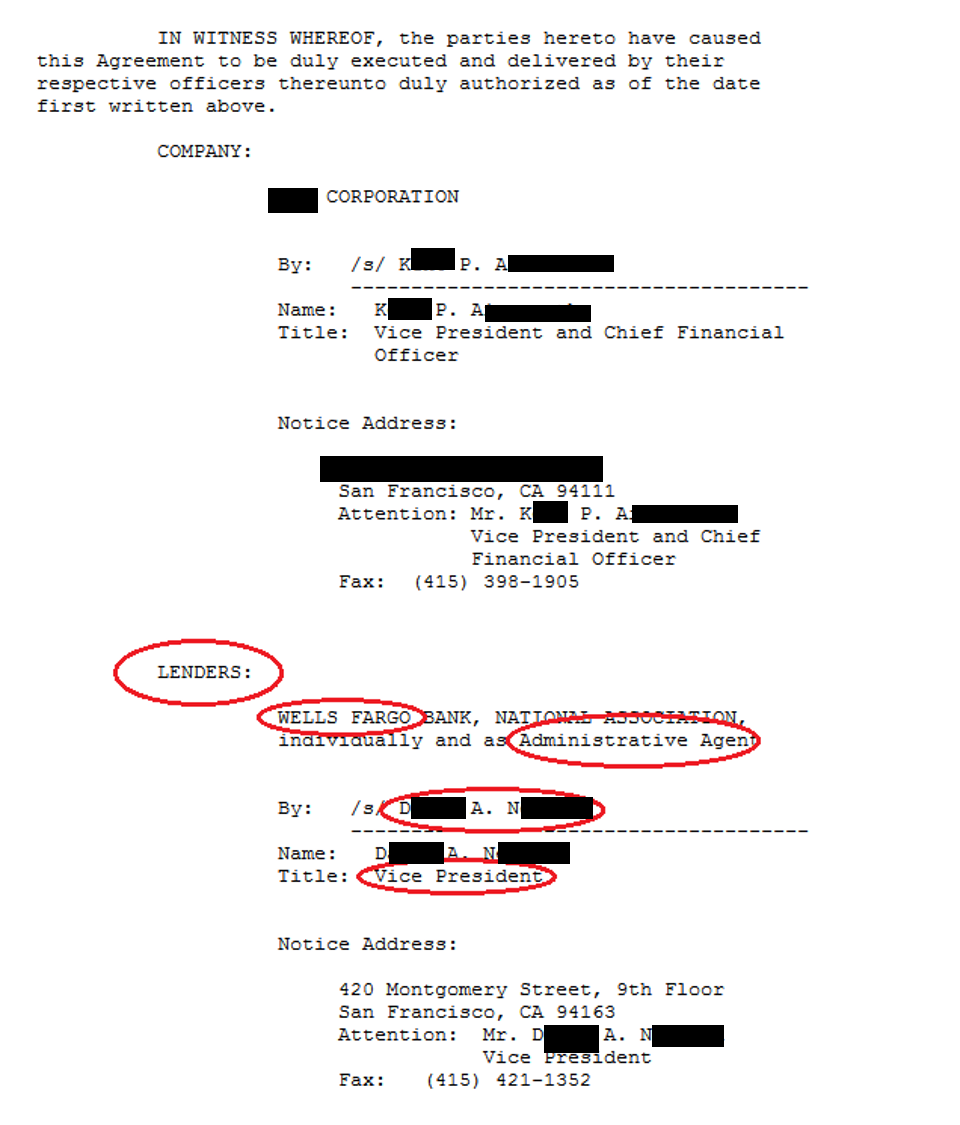
\includegraphics[scale=0.45]{../../Writeup/figures/signature_well_formated.png}
  }
  \end{column}% 
\hfill%
  \begin{column}{.6\textwidth}
    \begin{wideitemize}
      \item Loans considered ``material events''\\ \faArrowRight~ firms must file loan contracts to SEC
      \onslide<2->{
      \item Scrape all 8-K, 10-K, and 10-Q filings and use algorithm developed by Herpfer (2020) to obtain loan information:
      \begin{wideitemize}
          \item \textcolor{red}{Bank Name}
          %\item Bank Role
          \item \textcolor{red}{Person Name}
          %\item Person Title
        \end{wideitemize} }

      \onslide<3->{\item Obtain \textcolor{red}{personal relationships} between banker and clients \textcolor{red}{and} identify \textcolor{red}{bankers that switch} their employer.
      \item From 1996 to 2013, we retrieve some 20,000 bankers that switch 1,047 times. 
      \item \hyperlink{appendix_bankers}{\beamergotobutton{Quality-check}} }
    \end{wideitemize}
  \end{column}%
\end{columns}
\end{frame}
\note[itemize]{
\item DATA
\item An 8K can be any sort of announcement of significant corporate information. It's like a press release by the company. A 10K/Q is a formal annual/quarterly filing that contains the annual financial statements and lots of other information.
\item The data often gets a lot of quesitons - this is not the place to fight this battle. If someone gets aggressive tell them "we follow three papers published in top journals that provide extensive quality checks, happy to discuss details later but want to focus on novel part"
}

%%%%% EXAMPLE
\begin{frame}{Data - Example} \vfill
\begin{figure}[T]  \begin{center}
  \( \begin{array}{cccccc} 
  Yr & Banker & Bank & Firm & Banker~hired & Client~portfolio  \\ \toprule
  2000 & Joe & BofA & GM & 0 & GM \\
  2001 & Joe & BofA & - & 0 & GM \\
  2002 & Joe & BofA & - & 0 & GM  \\
  \marktopleft{a0}2003 & Joe & BofA & HP & 0 & GM;~HP  \\
  2005 & Joe & JPMorgan & GM & 1 & GM;~HP\markbottomright{a0}{red}  \\
  2006 & Joe & JPMorgan & - & 0 & GM;~HP  \\
  \multicolumn{6}{c}{\ldots} \\
  2009 & Joe & JPMorgan & 3M & 0 & GM;~HP;~3M \\ \bottomrule 
  \end{array} \)  \vfill 
\end{center} \end{figure} \vfill
 \only<2>{\centering In 2005 banker Joe switches from BofA to JPMorgan. \\ Crucially, he will bring over his \textcolor{red}{``personal relationships''} to GM and HP.  \vfill \tikz[overlay,remember picture,inner sep=1pt]
\node[draw=red,rounded corners,fit=(marker-a0-a.north west) (marker-a0-b.south east)] {};} 
\end{frame}

%%%%%%%%%%%%%%%%%%%%%%%%%%%%%%%%%%%%%%%%%%%%%%%%%%%%%%%%%%%%%%%%%%%%%%
%%%%%%%%%%%%%%%%%%%%%%%%%%%%%%%%%%%%%%%%%%%%%%%%%%%%%%%%%%%%%%%%%%%%%%
\begin{transitionframe}
  \begin{center}
    \Huge ~  \\ Finding I \\ ~ \\ Which bankers are being poached?
  \end{center}
\end{transitionframe}
%%%%%%%%%%%%%%%%%%%%%%%%%%%%%%%%%%%%%%%%%%%%%%%%%%%%%%%%%%%%%%%%%%%%%%
%%%%%%%%%%%%%%%%%%%%%%%%%%%%%%%%%%%%%%%%%%%%%%%%%%%%%%%%%%%%%%%%%%%%%% 
%%%%%%%%%%%%%%%%%%%%%%%%%%%%%%%%%%%%%%%
% MAIN FINDINGS 1 - CLIENT PORTFOLIO
%%%%%%%%%%%%%%%%%%%%%%%%%%%%%%%%%%%%%%%
\section{Main Findings}
\begin{frame}{Finding I - Bankers with a more valuable client portfolio are more likely to switch} 

 \begin{columns}[c] % align columns
  \begin{column}{.55\textwidth}
        \resizebox{\textwidth}{!}{ \centering 
  \begin{tabular*}{\hsize}{@{\hskip\tabcolsep\extracolsep\fill}l*{2}{c}} \toprule 
  Dep. variable:  &\multicolumn{2}{c}{Banker hired (\%)}  \\ \midrule
  \marktopleft{a1}\#Clients-Total\(_{t-1}\)&     0.15***         \\
             &   (3.87)   &\markbottomright{a1}{red} \\
 \marktopleft{a2}\#Clients-Single contact\(_{t-1}\)& &  0.58*** \\
    & &  (4.14) \\
    \#Clients-Mult. contact\(_{t-1}\)&            &   -0.14** \\
    &&  (-2.10)  \markbottomright{a2}{red} \\
      \midrule Observations    &  39,992   &    39,992  \\
      R-squared       &    0.21   &     0.22 \\
      \midrule Bank-Year FE    & Yes   &      Yes  \\
      \bottomrule
      \end{tabular*} 
  } \end{column}% 
\hfill%
  \begin{column}{.45\textwidth}
     \only<1>{\textcolor{red}{Dependent var.:} Indicator for first year banker appears at new bank \\ \vspace{.2cm}
     \textcolor{red}{Explanatory vars.:} \#Clients that a banker has in her portfolio at switch \\ \vspace{.2cm}  }

     \only<2>{\centering Bankers that have \textcolor{red}{\\relationships to more clients} \\ are more likely to switch \\ \vspace{.4cm} 

     +1 SD \#Clients (4.29) \\ increases the chance that this banker switches to a competing bank by 0.65\% \\ (+40\% of the unconditional likelihood)}

     \only<3>{\centering  This is especially true for single-contact clients where the banker is their only relationship } %we later show they are more likely to follow these banker} 
    
    \only<4>{\centering The same holds for \#Deals at the old bank}
  
    \only<5>{ \begin{center} \large \textcolor{red}{\textbf{Banks seem to recognize the \\ ability of bankers to bring new business \\ \vspace{.2cm} and are strategic in \\hiring the most valuable ones}} \end{center} }

  \end{column}%
\end{columns} 

\only<2>{\tikz[overlay,remember picture,inner sep=1pt] \node[draw=red,rounded corners,fit=(marker-a1-a.north west) (marker-a1-b.south east)] {};}
\only<3>{\tikz[overlay,remember picture,inner sep=1pt] \node[draw=red,rounded corners,fit=(marker-a2-a.north west) (marker-a2-b.south east)] {};}
\end{frame}


%%%%%%%%%%%%%%%%%%%%%%%%%%%%%%%%%%%%%%%%%%%%%%%%%%%%%%%%%%%%%%%%%%%%%%
%%%%%%%%%%%%%%%%%%%%%%%%%%%%%%%%%%%%%%%%%%%%%%%%%%%%%%%%%%%%%%%%%%%%%%
\section{ Finding II - Initiation and deal volume}
\begin{transitionframe}
  \begin{center}
    \Huge ~\\ Finding II \\ ~ \\ Does the new bank profit \\ from the switch?
  \end{center}
\end{transitionframe}
%%%%%%%%%%%%%%%%%%%%%%%%%%%%%%%%%%%%%%%%%%%%%%%%%%%%%%%%%%%%%%%%%%%%%%
%%%%%%%%%%%%%%%%%%%%%%%%%%%%%%%%%%%%%%%%%%%%%%%%%%%%%%%%%%%%%%%%%%%%%%

%%%%%%%%%%%%%%%%%%%%%%%%%%%%%%%%%%%%%%%
% EXAMPLE 2 - INITIATION
%%%%%%%%%%%%%%%%%%%%%%%%%%%%%%%%%%%%%%%
\begin{frame}{The perspective of the bank}
\begin{wideitemize}
  \item Take the perspective of the bank that hires the banker
  \item Define \textcolor{red}{$Rel\_acq$} as an indicator for all firms with whom the hired banker has a connection from past employment, i.e., for whom the bank \textcolor{red}{``acquires''} a relationship
  \item Define \textcolor{red}{$Initiation$} as the first time, or the first time in more than 5 years, that a bank closes a deal with a firm 
  \item \textcolor{red}{$Deals$} will be either syndicated loans (Dealscan), bond or SEO underwriting, or M\&A advisory (CapitalIQ) for which the volume is available
\end{wideitemize}

\vspace{.3cm}
\only<1> { \large ~ \\ ~ \\ ~ \\}
\only<2> {
{ \large \begin{center} \textcolor{red}{\textbf{Do bankers succeed in \\ bringing their previous clients with them at the new bank?} } \end{center} } }
\end{frame} 

\begin{frame}{Finding IIa - Initiation}
 \begin{columns}[c] % align columns
  \begin{column}{.7\textwidth}
\setbeamercovered{invisible}
\makebox[\linewidth][l]{
\begin{tabular}{l c <{\onslide<2->}c<{\onslide<3->}c<{\onslide<4->}c<{\onslide}}
 \toprule 
  Dep. variable:  & \multicolumn{4}{c}{Initiation}  \\ \midrule
   Rel\_acq & 0.07** &0.09** &   0.13***&      0.14*** \\
   &   (2.37)   &   (2.38)   &   (3.58)   &   (3.80)   \\
    \midrule Observations    &  861,444   &  861,444   &  861,444   &  861,444    \\
R-squared &     0.03   &     0.08   &     0.10   &     0.42 \\
\midrule Year FE & Yes   &Yes   &Yes   &       No      \\
Firm \& Bank FE         &Yes&No   &       No   &       No      \\
\marktopleft{a1}Firm-Bank FE    &  No   &Yes  \markbottomright{a1}{red} &      Yes   &      Yes \\
\marktopleft{a2}Bank-Year FE    & No   &No   &      Yes\markbottomright{a2}{red}   &      Yes  \\
\marktopleft{a3}Firm-Year FE    &No    &No    &No   &Yes\markbottomright{a3}{red}  \\   \bottomrule
\end{tabular}
} \end{column} 
\hfill%
\begin{column}{.25\textwidth} \begin{center}
  \only<1>{Acquiring a personal contact to a client makes it \textcolor{red}{7\% more likely to initiate a new business relationship} with him \\ ~ \\ This is economically meaningful, compared to the unconditional probability of 5.2\%}

  \only<2>{\textcolor{red}{Firm-Bank FEs} absorb time-unvarying characteristics on \textcolor{red}{the firm \& bank level} \\ (size, culture, geography) and \textcolor{red}{pair-specific} characteristics (e.g., bank specialized in the firm's industry)}

  \only<3>{\textcolor{red}{Bank-Year FEs} absorb \textcolor{red}{changes in loan supply}, e.g., a bank is hiring bankers because it wants to expand its operations}

  \only<4>{\textcolor{red}{Firm-Year FEs} absorb \textcolor{red}{changes in loan demand}, e.g., a firm taking out new loans to finance an acquisition}

  \only<5>{\large \textbf{\textcolor{red}{Bankers are successful in bringing their old clients to the new bank}}}
  \end{center} \end{column}
  \end{columns}
\only<2>{\tikz[overlay,remember picture,inner sep=1pt] \node[draw=red,rounded corners,fit=(marker-a1-a.north west) (marker-a1-b.south east)] {};}
\only<3>{\tikz[overlay,remember picture,inner sep=1pt] \node[draw=red,rounded corners,fit=(marker-a2-a.north west) (marker-a2-b.south east)] {};}
\only<4>{\tikz[overlay,remember picture,inner sep=1pt] \node[draw=red,rounded corners,fit=(marker-a3-a.north west) (marker-a3-b.south east)] {};}
\end{frame}
\note[itemize]{
\item INITIATION FIXED EFFECTS - SLOW!
  \item It could be that firms change banks not because of their bankers switching, but because of particular characteristics of the new bank. 
  \item To mitigate this we introduce a firm-bank FE -> We essentially compare the same firm-bank pair over time, before and after a banker with a prior relationship to the firm switches to the bank. 
  \item It could also be that a bank is hiring new bankers and initiating new client relationships because it wants to expand its operations. To account for this we introduce bank-time FEs. We are now essentially comparing for the same bank, the probability of initiating a relationship with new clients for which a relationship has been acquiring to new clients for which no relationship has been acquired.
  \item Finally, it could also be that firms are shopping for loans because they need funding for a new investment or acquisition. To account for that we include firm-yr-FEs. Now we are comparing the propensity of the same firm to borrow from a bank that has a personal relationship as opposed to one that has no relationship
}

%%%%%%%%%%%%%%%%%%%%%%%%%%%%%%%
%%% DEAL VOLUME 
%%%%%%%%%%%%%%%%%%%%%%%%%%%%%%%%%%

\begin{frame}{Finding IIb - Deal volume}
 \begin{columns}[c] % align columns
  \begin{column}{.7\textwidth}
\makebox[\linewidth][l]{
\begin{tabular}{l cccc}
 \toprule 
  Dep. variable:  & \multicolumn{4}{c}{Log Deal Volume}  \\ \midrule
   Rel\_acq        &     0.66***&     0.72***&     0.62***&    \marktopleft{a1} 0.35*** \\
   &    (6.78)   &   (3.79)   &   (4.58)   &   (3.85)   \\
    \midrule Observations    &   809,173   &  809,173   &  809,173   &  809,173     \\
R-squared &     0.07   &     0.14   &     0.16   &     0.51~~~   \\
\midrule Year FE & Yes   &Yes   &Yes   &       No      ~~~\\
Firm \& Bank FE         &Yes&No   &       No   &       No~~~      \\
Firm-Bank FE    &  No   &Yes  &      Yes   &      Yes ~~~\\
Bank-Year FE    & No   &No   &      Yes   &      Yes  ~~~\\
Firm-Year FE    &No    &No    &No   &Yes  ~~\markbottomright{a1}{red}\\   \bottomrule
\end{tabular}
} \end{column} 
\hfill%
\begin{column}{.25\textwidth} \begin{center}
  \only<1>{But do these new clients also bring deals for the bank?}
  \only<2>{+1 SD in Rel\_acq (0.06) correlates to an \textcolor{red}{increase in deal volume of ca. 2\%}}
%17m USD for the mean deal 

%After a banker switches, the new lender’s \textcolor{red}{deal volume with the banker’s relationship clients increases by 35\%}}

  \only<3>{The boost in deals is attributable to both \textcolor{red}{syndicated lending \& bond underwriting}. \\ ~ \\ The relationships acquired by the bank are \textcolor{red}{long lasting} and extend for years after the first deal.}
  
  \only<4>{Robust to tight FE structure, to different definitions of $Rel\_acq$ (5yrs and absorptive), and to dropping the first observation of the banker at the new bank.}

  \only<5>{\textbf{\textcolor{red}{ \large The relationships a lender can acquire by poaching a banker have significant commercial value.}}}

  \end{center} \end{column}
  \end{columns}
\only<2>{\tikz[overlay,remember picture,inner sep=1pt] \node[draw=red,rounded corners,fit=(marker-a1-a.north west) (marker-a1-b.south east)] {};}
\end{frame}
\note[itemize]{
  \item  
}


%%%%%%%%%%%%%%%%%%%%%%%%%%%%%%%%%%%%%%%%%%%%%%%%%%%%%%%%%%%%%%%%%%%%%%
%%%%%%%%%%%%%%%%%%%%%%%%%%%%%%%%%%%%%%%%%%%%%%%%%%%%%%%%%%%%%%%%%%%%%%
\section{Finding III - Labor market frictions spillover}
\begin{transitionframe}
  \begin{center}
    \Huge ~ \\ Finding III \\ ~ \\ Bankers' labor market frictions \\ spill overs into capital markets 
  \end{center}
\end{transitionframe}

\begin{frame}{Labor market frictions}
\textcolor{red}{Do labor market frictions spill over into financial markets?}
\begin{wideitemize}
  \item Use gender as an example
  \item Particularly important in financial services where there are large gaps between the representation of men and women in leadership positions in banks (IMF, 2018)
  % https://blogs.imf.org/2018/09/19/women-in-finance-an-economic-case-for-gender-equality/
  
  \item E.g., in our sample, none of the banks have a female CEO and only 19\% of bankers are women

  \item Use labor discrimination lawsuits and an indicator for not having female directors as a proxy for a bank culture that is unfriendly towards women
\end{wideitemize} \vspace{.5cm}
\only<1>{~\\~\\~\\}

\only<2>{
\begin{center} \faArrowRight~ Expect female bankers to \textcolor{red}{leave unfriendly banks} \\  and take their client relationships with them. \end{center}
}
\end{frame}
\note[itemize]{
\item LABOR MARKET FRICTION / GENDER
  \item \textcolor{blue}{CH: Pitch: Now we focus on one particular friction in the labor market. This is the current frontier of the paper. There is still a lot that we have to do here but we have initial exciting results focusing on a topic that has recently received a lot of attention. Gender. }
  \item \textcolor{blue}{CH: Pitch: Particularly relevant in financial services (pay gap largest, lawsuits, low representation females)}
  \item \textcolor{blue}{CH: Pitch: Do we observe interaction? Would expect female bankers to leave unfriendly banks. Proxy using lawsuits and female directors}
}

\begin{frame}{Finding IIIa - Labor market frictions}
\begin{columns}[c] % align columns
  \begin{column}{.5\textwidth}
\setbeamercovered{invisible} \makebox[\linewidth][l]{
\scalebox{0.7}{
\begin{tabular}{l c <{\onslide<2->}c<{\onslide<3->}c<{\onslide}}
 \toprule 
  Dep. variable:  & \multicolumn{3}{c}{Banker hired (\%)}  \\ \midrule
Empl. discrimination\(_{t-1}\) $\times$ Female &  2.79   &  &  \\
 &   (0.96) & &     \\
Empl. discrimination\(_{t-1}\)&   -22.92*  &    &  \\
                &  (-1.76)   &      &            \\
Gender discrimination\(_{t-1}\) $\times$ Female &  &    4.71** & \\
                &            &   (2.08)   &     \\
Gender discrimination\(_{t-1}\)&            &   -17.90  &            \\
                &            &  (-1.21)   &  \\
No female director\(_{t-1}\) $\times$ Female &    &  &  3.06*         \\
                     &  &  &      (1.74) \\
No female director\(l_{t-1}\)&      &  &   0.88 \\
&      &  &  (0.76) \\
% Female director\(_{t-1}\) $\times$ Female &   &  &    -2.82*  \\
%                                               & &  &  (-1.98)   \\
% Female director\(_{t-1}\) & & &   -0.71   \\
%                   &   & &  (-0.75)   \\
Female        &     0.42   &     0.68  &         0.72  \\
                &   (0.23)   &   (0.43)   &     (0.86)  \\
\midrule
Observations    &    3,308   &    3,308   &      552   \\
R-squared       &     0.86   &     0.86   &     0.94   \\
\midrule Prev. Bank FE   & Yes   & Yes   &      Yes   \\
Bank and Year FE&      Yes   &      Yes   &    Yes   \\
Banker controls &       No   &      Yes   &    Yes   \\
\bottomrule
\end{tabular} } } \end{column} 
\hfill%
\begin{column}{.4\textwidth} \begin{center}
  \only<1>{Employment discrimination lawsuits have a positive but insignificant effect on female banker turnover}

  \only<2>{\textcolor{red}{Gender discrimination lawsuits} have, as expected, a strong positive effect on the probability of female bankers leaving the bank...}

  \only<3>{... the same holds for having no women on the board of directors.}

  \only<4>{\vfill \large \textbf{\textcolor{red}{Banks with a less friendly culture towards women are more likely to lose female bankers.}} \vfill}
  \end{center} \end{column}
  \end{columns}
\end{frame}

\begin{frame}{Finding IIIb - Capital market implications of the labor market frictions}

\begin{columns}[c] % align columns
  \begin{column}{.5\textwidth}
\setbeamercovered{invisible} \makebox[\linewidth][l]{
\scalebox{.9}{
\begin{tabular}{l c <{\onslide<2->}cc<{\onslide}}
 \toprule 
 Dep. variable: &\multicolumn{3}{c}{Log Deal Volume} \\
 &\multicolumn{1}{c}{All}&\multicolumn{1}{c}{Lawsuit}&\multicolumn{1}{c}{No lawsuit}\\\cmidrule(lr){2-2}\cmidrule(lr){3-3}\cmidrule(lr){4-4}
 &\multicolumn{1}{c}{(1)}   &\multicolumn{1}{c}{(2)}   &\multicolumn {1}{c}{(3)}   \\
\midrule
Rel\_acq $\times$ Female &     0.19   &    -0.40   &     0.84* \\
                &   (0.44)   &  (-0.76)   &   (1.85)   \\
\addlinespace
Rel\_acq &     0.36***&     0.55*  &     0.35***\\
                &   (3.75)   &   (2.26)   &   (3.27)   \\
\midrule
Observations    &  809,173   &   79,918   &  647,276   \\
R-squared       &     0.51   &     0.61   &     0.53   \\
\midrule 
Firm-Bank FE    &      Yes   &      Yes   &      Yes   \\
Bank-Year FE    &      Yes   &      Yes   &      Yes   \\
Firm-Year FE    &      Yes   &      Yes   &      Yes   \\
\bottomrule
\end{tabular} } } \end{column} 
\hfill%
\begin{column}{.4\textwidth} \begin{center}
  \only<1>{In the full sample there is no significant difference between the deal volume generated with relationships of female and male bankers}

  \only<2>{... however, banks that are \textcolor{red}{not} involved in a gender discrimination lawsuit, profit more when a woman is hired.}

  \only<3>{\textbf{\textcolor{red}{\large It seems that, on the margin, \\ having a female friendly culture \\ allows banks to hire the more valuable female bankers.}}}
  \end{center} \end{column}
  \end{columns}

\end{frame}

\begin{frame}{Conclusion}
We investigate the \textcolor{red}{role of individual bankers} in the formation of bank-borrower relationships.
\begin{wideitemize}
  \item After bankers switch to a new bank, their former clients are 3$\times$ as likely to initiate a new lending relationship with that lender, compared to the unconditional mean
  \item The newly acquired borrowers bring an increase in deal volume across various product groups, and this increase is long-lasting
  \item We provide one specific application using gender culture as labor market friction: Female bankers are leaving banks with female-unfriendly cultures and shift significant business to competing banks.
\end{wideitemize}

\end{frame}
\begin{transitionframe}
  \begin{center}
    \Huge Thank you!
  \end{center}
\end{transitionframe}

% %%%%%%%%%%%%%%%%%%%%%%%%%%%%%%%%%%%%%%%%%%%%%%%%%%%%%%%%%%%%%%%%%%%%%%
% %%%%%%%%%%%%%%%%%%%%%%%%%%%%%%%%%%%%%%%%%%%%%%%%%%%%%%%%%%%%%%%%%%%%%%
\appendix
\begin{transitionframe}
  \begin{center}
    \Huge Appendix
  \end{center}
\end{transitionframe}
% %%%%%%%%%%%%%%%%%%%%%%%%%%%%%%%%%%%%%%%%%%%%%%%%%%%%%%%%%%%%%%%%%%%%%%
% %%%%%%%%%%%%%%%%%%%%%%%%%%%%%%%%%%%%%%%%%%%%%%%%%%%%%%%%%%%%%%%%%%%%%%

\begin{frame}[label=appendix_bankers]{Data - Individual bankers: Quality assurance}
Randomly sample 100 contracts to check quality of data:
\begin{wideitemize}
  \item 65\% of contracts feature signatures, other contracts are dropped
  \item 80\% of signatories are extracted successfully
\end{wideitemize}
\vspace{.3cm}
Talk to various bankers in commercial lending
\begin{wideitemize}
  \item Authorization of signature only for high ranking bankers
  \item Bankers that sign are the ones negotiating
  \item Titles are at the level of junior seniors
  \item LinkedIn search: Relationship bankers, commercial bankers     
\end{wideitemize}
\hfill \hyperlink{data_bankers}{\beamergotobutton{Back}}
\end{frame}


\end{document}
% %%%%%%%%%%%%%%%%%%%%%%%%%%%%%%%%%%%%%%%
% % DATA 2 - INITIATION SUMMARY STATS
% %%%%%%%%%%%%%%%%%%%%%%%%%%%%%%%%%%%%%%%
% \begin{frame}{Data II - Summary statistics}
% \makebox[\linewidth][c] {\centering
%   \begin{tabular}{lcccccc}
%                         &           N&         p25&        mean&         p50&         p75&          sd\\
% \midrule
% \marktopleft{a1}Initiation\_strict (\%)&     972,090&        0.00&        4.74&        0.00&        0.00&       21.25\markbottomright{a1}{red}\\
% \marktopleft{a2}Initiation (\%)     &     972,090&        0.00&        5.19&        0.00&        0.00&       22.19\markbottomright{a2}{red}\\
% \marktopleft{a3}Rel\_acq (\%)       &     972,090&        0.00&        2.93&        0.00&        0.00&       16.86\markbottomright{a3}{red}\\
% \marktopleft{a4}Rel\_acq\(^{5yr}\) (\%)&     958,303&        0.00&        1.53&        0.00&        0.00&       12.28\\
% Rel\_acq\(^{abs}\) (\%)&     946,223&        0.00&        0.27&        0.00&        0.00&        5.23\markbottomright{a4}{red}\\
% \marktopleft{a5}Volume - All deals  &     972,090&        0.00&       75.86&        0.00&        0.00&      806.00\markbottomright{a5}{red}\\
% \marktopleft{a6}Volume - Bonds      &     972,090&        0.00&       25.61&        0.00&        0.00&      376.80\\
% Volume - SEOs       &     972,090&        0.00&        5.15&        0.00&        0.00&      139.88\\
% Volume - Synd. Loans&     972,090&        0.00&       38.25&        0.00&        0.00&      490.65\markbottomright{a6}{red}\\
% \bottomrule \vspace{.2cm}
%   \end{tabular}
% }
% \centering 
% \only<1>{Collapse dataset at the \textcolor{red}{bank $\times$ firm $\times$ year} level \& add bank-firm deals \\ (loans, bonds, and SEOs) w/o banker information \\ \vspace{.1cm}~ \faArrowRight~ Total of 50k loans, 25k bonds, and 13k SEOs} %(some deals counted multiple times if they are closed jointly by more than one bank)
% \only<2>{Initiation\_strict identifies \textcolor{red}{1st time interaction} between a bank and a firm \\~  \\ \vspace{.1cm}~ \tikz[overlay,remember picture,inner sep=1pt] \node[draw=red,rounded corners,fit=(marker-a1-a.north west) (marker-a1-b.south east)] {};}
% \only<3>{Initiation also includes deals with \textcolor{red}{stale clients} (no deal in more than 5yrs) \\~  \\ \vspace{.1cm}~ \tikz[overlay,remember picture,inner sep=1pt] \node[draw=red,rounded corners,fit=(marker-a2-a.north west) (marker-a2-b.south east)] {};}
% \only<4>{Rel\_acq takes the value of 1 for \textcolor{red}{all pairs of new\_bank$\times$old\_client$\times$yr}, \\ for all years after the switch  \\ \vspace{.1cm}~ \tikz[overlay,remember picture,inner sep=1pt] \node[draw=red,rounded corners,fit=(marker-a3-a.north west) (marker-a3-b.south east)] {};}
% \only<5>{Rel\_acq${^{5yr}}$ and Rel\_acq$^{abs}$ take the value of 1, \\ for \textcolor{red}{5-yrs and 1-yr after the switch} and set to missing afterwards  \\ \vspace{.1cm}~ \tikz[overlay,remember picture,inner sep=1pt] \node[draw=red,rounded corners,fit=(marker-a4-a.north west) (marker-a4-b.south east)] {};}
%  \only<6>{Volume - All deals is \textcolor{red}{the sum of all deals} (loans, bonds, SEOs) that \\ a bank closes with a borrower within a year (in USDmm)  \\ \vspace{.1cm}~ \tikz[overlay,remember picture,inner sep=1pt] \node[draw=red,rounded corners,fit=(marker-a5-a.north west) (marker-a5-b.south east)] {};}
%   \only<7>{Volume of deals that a bank closes during a year \textcolor{red}{by deal type} (UDSmm) \\~  \\ \vspace{.1cm}~  \tikz[overlay,remember picture,inner sep=1pt] \node[draw=red,rounded corners,fit=(marker-a6-a.north west) (marker-a6-b.south east)] {};}
% \end{frame}

% \note[itemize]{
% \item The deals don't sum up because the data is at the banker-bank level, i.e., a deal can be counted multiple times at different banks 
% \item The median is 0 all the time because you fill in the gaps and treat years with no deals as explicit zero deals
%   \item Conditional on having a deal, the size of bonds (26k) is 1.5x larger than that of synd loans (50k)
%   \item SEOs are the smallest of the lot (12.8k)
% }

% %%%%%%%%%%%%%%%%%%%%%%%%%%%%%%%%%%%%%%%
% % MAIN FINDINGS 2.1 - INITIATION
% %%%%%%%%%%%%%%%%%%%%%%%%%%%%%%%%%%%%%%%
% \begin{frame}[label=finding2_init]{Finding IIa - Does the new bank profit from the switch?}
%  \begin{columns}[c] % align columns
%   \begin{column}{.65\textwidth}
%     \resizebox{\textwidth}{!}{ \centering 
%       \begin{tabular*}{\hsize}{@{\hskip\tabcolsep\extracolsep\fill}l*{4}{c}}
%  \toprule Dep. variable: &\multicolumn{4}{c}{Initiation}                                  \\\cmidrule(lr){2-5}
%                 &\multicolumn{1}{c}{(1)}   &\multicolumn{1}{c}{(2)}   &\multicolumn{1}{c}{(3)}  &\multicolumn{1}{c}{(4)}  \\
% \midrule
% \marktopleft{a1}Rel\_acq        &     0.07** &     0.09** & 0.13*** &    0.14***   \\
%                 &   (2.37)   &   (2.38)  &      (3.58)  &   (3.80)\markbottomright{a1}{red}   \\
% \midrule
% Observations    &  861,444   &  861,444   &  861,444   &  861,444   \\
% R-squared       &     0.03   &     0.08 &     0.10    &     0.42     \\
% \midrule 
% Year FE &      Yes   &      Yes   & Yes   &        No    \\
% Firm FE         &      Yes   &       No   &    No   &      No     \\
% \marktopleft{a2}Firm-Bank FE    &       No   &      Yes   &      Yes   &      Yes \\
% Bank-Year FE    &       No   &       No   &      Yes  &    Yes \\ 
% Firm-Bank FE    &       No   &      No   &      No  &      Yes\markbottomright{a2}{red}  \\ \bottomrule
% \end{tabular*}%
%   } \end{column}% 
% \hfill%
%   \begin{column}{.3\textwidth} 
%   \only<2>{\centering  Probability of initiating contact with new firm \\ \textcolor{red}{increases after the \\ bank acquires a personal relationship} \\ \vspace{.2cm} This corresponds to \\ 1.5x - 3x the average unconditional probability of initiation \tikz[overlay,remember picture,inner sep=1pt] \node[draw=red,rounded corners,fit=(marker-a1-a.north west) (marker-a1-b.south east)] {}; }
%   \only<3>{\centering Finding holds under \\ \textcolor{red}{tight FE structure}: \\ Bank $\times$ Year (supply), \\ Firm $\times$ Year (demand), and \\ Firm $\times$ Bank FEs (geographic proximity, compatible strategy etc.) \tikz[overlay,remember picture,inner sep=1pt] \node[draw=red,rounded corners,fit=(marker-a2-a.north west) (marker-a2-b.south east)] {};} 
%   \only<4>{\centering Findings remain virtually unchanged when we: \\ \vspace{.1cm} 
%   \begin{wideitemize} 
%     \item use stricter definition of initiation \\ \hyperlink{appendix_initiation}{\beamergotobutton{Table}}  
%     \item use different treatments (5-yrs \& absorptive) \\
%     \hyperlink{appendix_initiation_treat}{\beamergotobutton{Table}}  
%     \item drop first deal that banker signs at new bank \\
%     \hyperlink{appendix_initiation_nofirst}{\beamergotobutton{Table}}  
%     \end{wideitemize} }
%   \only<5>{\Large \centering The bank increases its borrower base by \textcolor{red}{winning over clients known to the banker}}
%       \end{column}%
% \end{columns}
%  \end{frame}

% \note[itemize]{
%  \item hammer down how strict this specification is: fill out sample, treat all relationships acquired as one from the moment the banker switches (explain why this is so conservative), include all relationships that are never brought over. Also, all other new clients that the bank acquires that are not in the bankers' portfolio count against us 
%   \item Result holds when using the various types of relationship acquired 
%   \item Result counts all years starting from the first time the banker appears at the new bank as rel\_acq=1
%   \item Firm-bank-FE accounts for e.g. time-invariant bank-firm-pair characteristics such as geographic proximity, compatible corporate culture and strategy 
%   \item Bank-year-FE account for changes in supply of lending at the bank level
%   \item Firm-year-FE account for changes in demand at the firm 
%   \item Standard errors are 2-way clustered around banks and bankers (adding time as the third dimension also doesn't change anything)
% }

% %%%%%%%%%%%%%%%%%%%%%%%%%%%%%%%%%%%%%%%
% % MAIN FINDINGS 2.2 - DEAL VOLUME
% %%%%%%%%%%%%%%%%%%%%%%%%%%%%%%%%%%%%%%%
% \begin{frame}[label=finding2_vol]{Finding IIb - Does the new bank profit from the switch?}
%  \begin{columns}[c] % align columns
%   \begin{column}{.65\textwidth}
%     \resizebox{\textwidth}{!}{ \centering 
% \begin{tabular*}{\hsize}{@{\hskip\tabcolsep\extracolsep\fill}l*{4}{c}}
% % \def\sym#1{\ifmmode^{#1}\else\(^{#1}\)\fi}
% \toprule
% Dep. variable: &\multicolumn{4}{c}{Log Deal Volume}                             \\\cmidrule(lr){2-5}
% &\multicolumn{1}{c}{(1)}   &\multicolumn{1}{c}{(2)}   &\multicolumn{1}{c}{(3)}   &\multicolumn{1}{c}{(4)} \\
% \midrule
% \marktopleft{a1}Rel\_acq        &     0.65***&     0.72***&     0.61***&     0.30***\\
%                &   (8.62)   &   (4.09)   &   (5.18)  &   (3.80)\markbottomright{a1}{red}  \\
% \midrule
% Observations    &  809,108   &  809,108   &  809,108   &  809,108   \\
% R-squared       &     0.07   &     0.14   &     0.16   &     0.51   \\
% \midrule
% Year FE &      Yes   &      Yes   &      Yes  &      No  \\
% Firm FE         &      Yes   &       No   &       No   &      No \\
% \marktopleft{a2}Firm-Bank FE    &       No   &      Yes   &      Yes   &      Yes \\
% Bank-Year FE    &       No   &       No   &      Yes  &    Yes \\ 
% Firm-Bank FE    &       No   &      No   &      No  &      Yes\markbottomright{a2}{red}\\
% \bottomrule
% \end{tabular*}%
%   } \end{column}% 
% \hfill%
%   \begin{column}{.3\textwidth} 
%   \only<2>{\centering The banks that acquire relationships when bankers switch \textcolor{red}{close more deals} with the new clients \\ \vspace{.2cm} For the median deal \\ (USD 300mm, conditional on closing), this corresponds to an increase of USD 2.1mm \tikz[overlay,remember picture,inner sep=1pt] \node[draw=red,rounded corners,fit=(marker-a1-a.north west) (marker-a1-b.south east)] {};}
%   \only<3>{\centering This holds under a \textcolor{red}{tight FE structure} \tikz[overlay,remember picture,inner sep=1pt] \node[draw=red,rounded corners,fit=(marker-a2-a.north west) (marker-a2-b.south east)] {};}
%    \only<4>{\centering Findings remain virtually unchanged when: \\ \vspace{.1cm} 
%       \begin{wideitemize} 
%     \item using different treatments (5-yrs \& absorptive)  
%      \\ \hyperlink{appendix_vol_treatment}{\beamergotobutton{Table}} 
%     \item looking at first deal and repeated interaction clients separately 
%      \\ \hyperlink{appendix_vol_first}{\beamergotobutton{Table}} 
%    \end{wideitemize}}
%   \only<5>{\Large \centering The bank \textcolor{red}{increases the volume of deals} with acquired clients \\ \vspace{.3cm} 
%   The increase covers \textcolor{red}{both syndicated lending and bonds} 
%      \\ \hfill \hyperlink{appendix_vol_dscan}{\beamergotobutton{Table}} }
%       \end{column}%
% \end{columns}
% \end{frame}

% \note[itemize]{
%   \item Here you drop relationships that don't come over
%   \item Treat all clients with whom you eventually make deals as rel\_acq from the first year after the switch
%   \item Not so much in SEO sample - consistent with investment banking business being separate from lending
%   \item Clearly, having FEs in there makes the comparison with the sample median not 100\% kosher
% }

% %%%%%%%%%%%%%%%%%%%%%%%%%%%%%%%%%%%%%%%
% % CONCLUSION / EXTENSIONS / NEXT STEPS
% %%%%%%%%%%%%%%%%%%%%%%%%%%%%%%%%%%%%%%%
% \section{Conclusion}
% \begin{frame}{Conclusion}
% In sum, bankers appear to be an important piece in explaining the creation of lending relationships. They \textcolor{red}{facilitate the matching} between firms and banks. \\ \vspace{.5cm} 
% \textcolor{red}{Open questions \& next steps:} 
% \begin{wideitemize}
%   \item \textcolor{red}{Identification} - Sources of exogenous variation in the probability of switching, e.g.,  restrictions in labor mobility or drop in bank performance/executive pay 
%   \item Role of \textcolor{red}{bank culture} - Are bankers more likely to leave banks with a ``toxic culture''?
%   \item Role of \textcolor{red}{demographics} - Are female bankers better at forming strong client relationships? Are they more or less likely to switch banks?
% \end{wideitemize}
% \end{frame}

% \begin{transitionframe}
%   \begin{center}
%     \Huge Thank you!
%   \end{center}
% \end{transitionframe}



% %%%%%%%%%%%%%%%%%%%%%%%%%%%%%%%%%%%%%%%%%%%%%%%%%%%%%%%%%%%%%%%%%%%
% \begin{frame}[label=appendix_tenure]{Finding Ia - Tenure}
%    \resizebox{.8\textwidth}{!}{ \centering 
% \begin{tabular*}{\hsize}{@{\hskip\tabcolsep\extracolsep\fill}l*{6}{c}}
% \toprule
%                 &\multicolumn{6}{c}{Pre-Switch Indicator (\%)}                                \\\cmidrule(lr){2-7}
%                 &\multicolumn{1}{c}{(1)}   &\multicolumn{1}{c}{(2)}   &\multicolumn{1}{c}{(3)}   &\multicolumn{1}{c}{(4)}   &\multicolumn{1}{c}{(5)}   &\multicolumn{1}{c}{(6)}   \\
% \midrule
% Tenure of banker (running)&     0.25** &     0.30***&            &            &            &            \\
%                 &   (2.57)   &   (3.07)   &            &            &            &            \\
 
% Max tenure of banker&            &            &     0.50***&     0.55***&            &            \\
%                 &            &            &   (4.90)   &   (5.66)   &            &            \\
 
% Tenure\(^{25\%-50\%}\)&            &            &            &            &     1.33***&     1.29***\\
%                 &            &            &            &            &   (3.39)   &   (3.44)   \\
 
% Tenure\(^{50\%-75\%}\)&            &            &            &            &     2.37***&     2.31***\\
%                 &            &            &            &            &   (4.02)   &   (3.66)   \\
 
% Tenure\(^{75\%-100\%}\)&            &            &            &            &     2.47***&     2.92***\\
%                 &            &            &            &            &   (3.05)   &   (3.54)   \\
% \midrule
% Observations    &   22,642   &   22,642   &    7,871   &    7,871   &   22,642   &   22,642   \\
% R-squared       &     0.23   &     0.31   &     0.26   &     0.38   &     0.23   &     0.31   \\
% \midrule Year FE &      Yes   &       No   &        Yes   &       No   &        Yes   &       No \\
% Bank FE         &      Yes   &       No   &        Yes   &       No   &        Yes   &       No \\
% Bank-Year FE    &      Yes   &       No   &        Yes   &       No   &        Yes   &       No \\
% \bottomrule
% \end{tabular*} }
% \hfill \hyperlink{finding1}{\beamergotobutton{Back}}
% \end{frame}

% %%%%%%%%%%%%%%%%%%%%%%%%%%%%%%%%%%%%%%%%%%%%%%%%%%%%%%%%%%%%%%%%%%%
% \begin{frame}[label=appendix_key]{Finding Ib - Key bankers}
%    \resizebox{.8\textwidth}{!}{ \centering 
% \begin{tabular*}{\hsize}{@{\hskip\tabcolsep\extracolsep\fill}l*{6}{c}}
% \toprule
%                 &\multicolumn{2}{c}{All bankers}&\multicolumn{2}{c}{Non-key}&\multicolumn{2}{c}{Key}  \\\cmidrule(lr){2-3}\cmidrule(lr){4-5}\cmidrule(lr){6-7}
%                 &\multicolumn{1}{c}{(1)}   &\multicolumn{1}{c}{(2)}   &\multicolumn{1}{c}{(3)}   &\multicolumn{1}{c}{(4)}   &\multicolumn{1}{c}{(5)}   &\multicolumn{1}{c}{(6)}   \\
% \midrule
% \%Bank deals by banker&     0.18***&     0.29***&     0.39***&     0.69***&     0.13***&     0.17***\\
%                 &   (8.08)   &   (9.91)   &   (7.25)   &   (9.28)   &   (4.36)   &   (3.62)   \\
% \midrule
% Observations    &   43,233   &   43,233   &   36,730   &   36,427   &    6,300   &    4,954   \\
% R-squared       &     0.24   &     0.30   &     0.18   &     0.22   &     0.57   &     0.71   \\
% \midrule Year FE &      Yes   &       No   &      Yes   &       No   &      Yes   &       No   \\
% Bank FE         &      Yes   &       No   &      Yes   &       No   &      Yes   &       No   \\
% Bank-Year FE    &       No   &      Yes   &       No   &      Yes   &       No   &      Yes   \\
% \bottomrule
% \end{tabular*}}
% \hfill \hyperlink{finding1}{\beamergotobutton{Back}}
% \end{frame}

% %%%%%%%%%%%%%%%%%%%%%%%%%%%%%%%%%%%%%%%%%%%%%%%%%%%%%%%%%%%%%%%%%%%%%%%%%%%
% %%%%%%%%%%%%%%%%%%%%%%%%%%%%%%%%%%%%%%%%%%%%%%%%%%%%%%%%%%%%%%%%%%%%%%%%%%%
% \begin{frame}[label=appendix_initiation]{Finding IIa - 1. Initiation strict}
%    \resizebox{.8\textwidth}{!}{ \centering 
%    \begin{tabular*}{\hsize}{@{\hskip\tabcolsep\extracolsep\fill}l*{6}{c}}
% \toprule
% Dep. variable: &\multicolumn{5}{c}{Initiation\_strict}                          \\\cmidrule(lr){2-6}
% &\multicolumn{1}{c}{(1)}   &\multicolumn{1}{c}{(2)}   &\multicolumn{1}{c}{(3)}   &\multicolumn{1}{c}{(4)}   &\multicolumn{1}{c}{(5)}   \\
% \midrule
% Rel\_acq        &     0.06** &     0.07** &     0.12***&            &            \\
%                 &   (2.42)   &   (2.51)   &   (4.11)   &            &            \\
 
% Rel\_acq\(^{5yr}\)&            &            &            &     0.11***&            \\
%                 &            &            &            &   (3.88)   &            \\
 
% Rel\_acq\(^{abs}\)&            &            &            &            &     0.06***\\
%                 &            &            &            &            &   (3.32)   \\
% \midrule
% Observations    &  861,444   &  861,444   &  861,444   &  847,106   &  834,470   \\
% R-squared       &     0.03   &     0.07   &     0.40   &     0.39   &     0.39   \\
% \midrule Year FE &      Yes   &      Yes   &       No   &       No   &       No   \\
% Firm FE         &      Yes   &       No   &       No   &       No   &       No   \\
% Firm-Bank FE    &       No   &      Yes   &      Yes   &      Yes   &      Yes   \\
% Bank-Year FE    &       No   &       No   &      Yes   &      Yes   &      Yes   \\
% Firm-Year FE    &       No   &       No   &      Yes   &      Yes   &      Yes   \\
% \bottomrule \end{tabular*}
% }
% \hfill \hyperlink{finding2_init}{\beamergotobutton{Back}}
% \end{frame}

% %%%%%%%%%%%%%%%%%%%%%%%%%%%%%%%%%%%%%%%%%%%%%%%%%%%%%%%%%%%%%%%%%%%%%%%%%%%
% \begin{frame}[label=appendix_initiation_nofirst]{Finding IIa - 2. Ignoring first deal}
%    \resizebox{.8\textwidth}{!}{ \centering 
%    \begin{tabular*}{\hsize}{@{\hskip\tabcolsep\extracolsep\fill}l*{6}{c}}
% \toprule
%                 Dep. variable: &\multicolumn{5}{c}{Initiation}                                  \\\cmidrule(lr){2-6}
%                 &\multicolumn{1}{c}{(1)}   &\multicolumn{1}{c}{(2)}   &\multicolumn{1}{c}{(3)}   &\multicolumn{1}{c}{(4)}   &\multicolumn{1}{c}{(5)}   \\
% \midrule
% Rel\_acq\_nofirst&     0.07** &     0.09** &     0.15***&            &            \\
%                 &   (2.35)   &   (2.35)   &   (3.88)   &            &            \\
 
% Rel\_acq\_nofirst\(^{5yr}\)&            &            &            &     0.14***&            \\
%                 &            &            &            &   (3.61)   &            \\
 
% Rel\_acq\_nofirst\(^{abs}\)&            &            &            &            &     0.09***\\
%                 &            &            &            &            &   (3.63)   \\
% \midrule
% Observations    &  858,844   &  858,844   &  858,844   &  844,504   &  834,668   \\
% R-squared       &     0.03   &     0.08   &     0.42   &     0.41   &     0.41   \\
% \midrule Year FE &      Yes   &      Yes   &       No   &       No   &       No   \\
% Firm FE         &      Yes   &       No   &       No   &       No   &       No   \\
% Firm-Bank FE    &       No   &      Yes   &      Yes   &      Yes   &      Yes   \\
% Bank-Year FE    &       No   &       No   &      Yes   &      Yes   &      Yes   \\
% Firm-Year FE    &       No   &       No   &      Yes   &      Yes   &      Yes   \\
% \bottomrule \end{tabular*}
% }
% \hfill \hyperlink{finding2_init}{\beamergotobutton{Back}}
% \end{frame}

% %%%%%%%%%%%%%%%%%%%%%%%%%%%%%%%%%%%%%%%%%%%%%%%%%%%%%%%%%%%%%%%%%%%%%%%%%%%
% \begin{frame}[label=appendix_initiation_treat]{Finding IIa - 3. Different treatments}
%    \resizebox{.8\textwidth}{!}{ \centering 
%    \begin{tabular*}{\hsize}{@{\hskip\tabcolsep\extracolsep\fill}l*{6}{c}}
% \toprule
%                   Dep. variable: &\multicolumn{5}{c}{Initiation}                                  \\\cmidrule(lr){2-6}
%                 &\multicolumn{1}{c}{(1)}   &\multicolumn{1}{c}{(2)}   &\multicolumn{1}{c}{(3)}   &\multicolumn{1}{c}{(4)}   &\multicolumn{1}{c}{(5)}   \\
% \midrule
% Rel\_acq        &     0.07** &     0.09** &     0.14***&            &            \\
%                 &   (2.37)   &   (2.38)   &   (3.80)   &            &            \\
 
% Rel\_acq\(^{5yr}\)&            &            &            &     0.12***&            \\
%                 &            &            &            &   (3.56)   &            \\
 
% Rel\_acq\(^{abs}\)&            &            &            &            &     0.07***\\
%                 &            &            &            &            &   (3.36)   \\
% \midrule
% Observations    &  861,444   &  861,444   &  861,444   &  847,106   &  834,470   \\
% R-squared       &     0.03   &     0.08   &     0.42   &     0.41   &     0.41   \\
% \midrule Year FE &      Yes   &      Yes   &       No   &       No   &       No   \\
% Firm FE         &      Yes   &       No   &       No   &       No   &       No   \\
% Firm-Bank FE    &       No   &      Yes   &      Yes   &      Yes   &      Yes   \\
% Bank-Year FE    &       No   &       No   &      Yes   &      Yes   &      Yes   \\
% Firm-Year FE    &       No   &       No   &      Yes   &      Yes   &      Yes   \\

% \bottomrule \end{tabular*}
% }
% \hfill \hyperlink{finding2_init}{\beamergotobutton{Back}}
% \end{frame}

% %%%%%%%%%%%%%%%%%%%%%%%%%%%%%%%%%%%%%%%%%%%%%%%%%%%%%%%%%%%%%%%%%%%%%%%%%%%
% %%%%%%%%%%%%%%%%%%%%%%%%%%%%%%%%%%%%%%%%%%%%%%%%%%%%%%%%%%%%%%%%%%%%%%%%%%%
% \begin{frame}[label=appendix_vol_treatment]{Finding IIb - 1. Volume - Different treatment}
%    \resizebox{.8\textwidth}{!}{ \centering 
%  \begin{tabular*}{\hsize}{@{\hskip\tabcolsep\extracolsep\fill}l*{6}{c}}
% \toprule
%                 &\multicolumn{6}{c}{Log Deal Volume}                                          \\\cmidrule(lr){2-7}
%                 &\multicolumn{1}{c}{(1)}   &\multicolumn{1}{c}{(2)}   &\multicolumn{1}{c}{(3)}   &\multicolumn{1}{c}{(4)}   &\multicolumn{1}{c}{(5)}   &\multicolumn{1}{c}{(6)}   \\
% \midrule
% Rel\_acq        &     0.65***&     0.72***&     0.61***&     0.30***&            &            \\
%                 &   (8.62)   &   (4.09)   &   (5.18)   &   (3.80)   &            &            \\
 
% Rel\_acq\(^{5yr}\)&            &            &            &            &     0.70***&            \\
%                 &            &            &            &            &   (6.07)   &            \\
 
% Rel\_acq\(^{abs}\)&            &            &            &            &            &     3.47***\\
%                 &            &            &            &            &            &   (6.58)   \\
% \midrule
% Observations    &  809,108   &  809,108   &  809,108   &  809,108   &  807,764   &  806,292   \\
% R-squared       &     0.07   &     0.14   &     0.16   &     0.51   &     0.16   &     0.16   \\
% \midrule Year FE &      Yes   &      Yes   &       Yes   &       Yes   &       Yes  &       Yes   \\
% Firm FE         &      Yes   &       No   &       No   &       No   &       No&       No   \\
% Firm-Bank FE    &       No   &      Yes   &      Yes   &      Yes   &      Yes   &      Yes   \\
% Bank-Year FE    &       No   &       No   &      Yes   &      Yes   &      Yes   &      Yes   \\
% \bottomrule
% \end{tabular*}
% }
% \hfill \hyperlink{finding2_vol}{\beamergotobutton{Back}}
% \end{frame}

% %%%%%%%%%%%%%%%%%%%%%%%%%%%%%%%%%%%%%%%%%%%%%%%%%%%%%%%%%%%%%%%%%%%%%%%%%%%
% \begin{frame}[label=appendix_vol_first]{Finding IIb - Volume 2. First vs. repeat deals}
%    \resizebox{.8\textwidth}{!}{ \centering 
%  \begin{tabular*}{\hsize}{@{\hskip\tabcolsep\extracolsep\fill}l*{6}{c}}
% \toprule
%                   Dep. variable: &\multicolumn{3}{c}{Volume - First deal}&\multicolumn{3}{c}{Volume - Repeat deals}\\\cmidrule(lr){2-4}\cmidrule(lr){5-7}
%                 &\multicolumn{1}{c}{(1)}   &\multicolumn{1}{c}{(2)}   &\multicolumn{1}{c}{(3)}   &\multicolumn{1}{c}{(4)}   &\multicolumn{1}{c}{(5)}   &\multicolumn{1}{c}{(6)}   \\
% \midrule
% Rel\_acq        &     0.81***&            &            &     1.29***&            &            \\
%                 &  (14.71)   &            &            &  (14.02)   &            &            \\
 
% Rel\_acq\(^{5yr}\)&            &     0.96***&            &            &     1.16***&            \\
%                 &            &  (13.83)   &            &            &  (10.65)   &            \\
 
% Rel\_acq\(^{abs}\)&            &            &     4.74***&            &            &     1.65***\\
%                 &            &            &  (11.62)   &            &            &   (6.43)   \\
% \midrule
% Observations    &  930,913   &  929,477   &  927,926   &  930,913   &  929,477   &  927,926   \\
% R-squared       &     0.18   &     0.22   &     0.83   &     0.38   &     0.35   &     0.37   \\
% \midrule Year FE &      Yes   &      Yes   &      Yes   &      Yes   &      Yes   &      Yes   \\
% Firm FE         &       No   &       No   &       No   &       No   &       No   &       No   \\
% Firm-Bank FE    &      Yes   &      Yes   &      Yes   &      Yes   &      Yes   &      Yes   \\
% Bank-Year FE    &      Yes   &      Yes   &      Yes   &      Yes   &      Yes   &      Yes   \\
% \bottomrule
% \end{tabular*}
% }
% \hfill \hyperlink{finding2_vol}{\beamergotobutton{Back}}
% \end{frame}


% %%%%%%%%%%%%%%%%%%%%%%%%%%%%%%%%%%%%%%%%%%%%%%%%%%%%%%%%%%%%%%%%%%%%%%%%%%%
% \begin{frame}[label=appendix_vol_dscan]{Finding IIb - Volume 3. Deal category}
%    \resizebox{.8\textwidth}{!}{ \centering 
%  \begin{tabular*}{\hsize}{@{\hskip\tabcolsep\extracolsep\fill}l*{6}{c}}
% \toprule
%                  Dep. variable: &\multicolumn{5}{c}{Log Deal Volume - Syndicated Loans}          \\\cmidrule(lr){2-6}
%                 &\multicolumn{1}{c}{(1)}   &\multicolumn{1}{c}{(2)}   &\multicolumn{1}{c}{(3)}   &\multicolumn{1}{c}{(4)}   &\multicolumn{1}{c}{(5)}   \\
% \midrule
% Rel\_acq        &     0.33***&     0.18   &     0.20** &            &            \\
%                 &   (4.62)   &   (1.40)   &   (2.04)   &            &            \\
 
% Rel\_acq\(^{5yr}\)&            &            &            &     0.37***&            \\
%                 &            &            &            &   (3.06)   &            \\
 
% Rel\_acq\(^{abs}\)&            &            &            &            &     1.84***\\
%                 &            &            &            &            &   (5.09)   \\
% \midrule
% Observations    &  574,769   &  574,769   &  574,769   &  574,032   &  573,293   \\
% R-squared       &     0.08   &     0.15   &     0.17   &     0.17   &     0.17   \\
% \midrule Year FE &      Yes   &      Yes   &      Yes   &      Yes   &      Yes   \\
% Firm FE         &      Yes   &       No   &       No   &       No   &       No   \\
% Firm-Bank FE    &       No   &      Yes   &      Yes   &      Yes   &      Yes   \\
% Bank-Year FE    &       No   &       No   &      Yes   &      Yes   &      Yes   \\
% \bottomrule
% \end{tabular*}
% }
% \hfill \hyperlink{finding2_vol}{\beamergotobutton{Back}}
% \end{frame}

% \begin{frame}[label=appendix_vol_bond]{Finding IIb - Volume 3. Deal category}
%    \resizebox{.8\textwidth}{!}{ \centering 
%  \begin{tabular*}{\hsize}{@{\hskip\tabcolsep\extracolsep\fill}l*{6}{c}}
% \toprule
%                 Dep. variable: &\multicolumn{5}{c}{Log Deal Volume - Bonds}                     \\\cmidrule(lr){2-6}
%                 &\multicolumn{1}{c}{(1)}   &\multicolumn{1}{c}{(2)}   &\multicolumn{1}{c}{(3)}   &\multicolumn{1}{c}{(4)}   &\multicolumn{1}{c}{(5)}   \\
% \midrule
% Rel\_acq        &     0.45***&     0.51***&     0.43***&            &            \\
%                 &   (5.31)   &   (5.02)   &   (6.66)   &            &            \\
 
% Rel\_acq\(^{5yr}\)&            &            &            &     0.45***&            \\
%                 &            &            &            &   (6.79)   &            \\
 
% Rel\_acq\(^{abs}\)&            &            &            &            &     2.52***\\
%                 &            &            &            &            &   (4.75)   \\
% \midrule
% Observations    &  288,896   &  288,896   &  288,896   &  287,820   &  286,598   \\
% R-squared       &     0.14   &     0.19   &     0.21   &     0.21   &     0.20   \\
% \midrule Year FE &      Yes   &      Yes   &      Yes   &      Yes   &      Yes   \\
% Firm FE         &      Yes   &       No   &       No   &       No   &       No   \\
% Firm-Bank FE    &       No   &      Yes   &      Yes   &      Yes   &      Yes   \\
% Bank-Year FE    &       No   &       No   &      Yes   &      Yes   &      Yes   \\
% \bottomrule
% \end{tabular*}
% }
% \hfill \hyperlink{finding2_vol}{\beamergotobutton{Back}}
% \end{frame}

% \begin{frame}[label=appendix_vol_seo]{Finding IIb - Volume 3. Deal category}
%    \resizebox{.8\textwidth}{!}{ \centering 
%  \begin{tabular*}{\hsize}{@{\hskip\tabcolsep\extracolsep\fill}l*{6}{c}}
% \toprule
%                 Dep. variable: &\multicolumn{5}{c}{Log Deal Volume - SEOs}                      \\\cmidrule(lr){2-6}
%                 &\multicolumn{1}{c}{(1)}   &\multicolumn{1}{c}{(2)}   &\multicolumn{1}{c}{(3)}   &\multicolumn{1}{c}{(4)}   &\multicolumn{1}{c}{(5)}   \\
% \midrule
% Rel\_acq        &     0.12   &     0.09   &     0.02   &            &            \\
%                 &   (0.94)   &   (0.30)   &   (0.06)   &            &            \\
 
% Rel\_acq\(^{5yr}\)&            &            &            &     0.11   &            \\
%                 &            &            &            &   (0.46)   &            \\
 
% Rel\_acq\(^{abs}\)&            &            &            &            &     0.61   \\
%                 &            &            &            &            &   (1.43)   \\
% \midrule
% Observations    &  201,741   &  201,741   &  201,741   &  201,330   &  200,873   \\
% R-squared       &     0.06   &     0.09   &     0.10   &     0.10   &     0.10   \\
% \midrule Year FE &      Yes   &      Yes   &       No   &      Yes   &      Yes   \\
% Firm FE         &      Yes   &       No   &       No   &       No   &       No   \\
% Firm-Bank FE    &       No   &      Yes   &      Yes   &      Yes   &      Yes   \\
% Bank-Year FE    &       No   &       No   &      Yes   &      Yes   &      Yes   \\

% \bottomrule
% \end{tabular*}
% }
% \hfill \hyperlink{finding2_vol}{\beamergotobutton{Back}}
% \end{frame}
% % Findings with different rel\_acq definitions
% % Findings with initiation interaction 


